\documentclass[10pt,utf8,presentation,notheorems,xcolor=dvipsnames,compress]{beamer}
\usepackage{doclad}

\setbeamertemplate{caption}[numbered]
\usepackage[labelsep=period]{caption}
\addto\captionsrussian{\renewcommand{\figurename}{Рисунок}}

\newcommand{\ov}{\overline}
\newcommand{\fr}{\cfrac}
\newcommand{\ti}{\times}
\newcommand{\ttt}{\theta}
\newcommand{\wt}{\widetilde}

\newcommand{\lwo}{\widetilde{\overline{\lambda}}}%лямбда волна черта
\newcommand{\lw}{\overline{\lambda}}%лямбда черта
\newcommand{\lo}{\lambda_{0}}%лямбда о
\newcommand{\lnw}{\overline{\lambda}_{\nu}} %лямбда ню черта

\newcommand{\mwo}{\widetilde{\overline{\mu}}} %мю волна черта
\newcommand{\mw}{\overline{\mu}} %мю черта
\newcommand{\mo}{\mu_{\o}} %мю  о
\newcommand{\mnw}{\overline{\mu}_{\nu}} %мю ню черта

\newcommand{\ow}{\overline{\omega}}%омега черта
\newcommand{\rw}{\overline{r}}%r черта
\newcommand{\rrw}{\overline{r'}}%r' черта
\newcommand{\ew}{\overline{e}}%e черта
\newcommand{\vw}{\overline{v}}%v черта
\newcommand{\pw}{\overline{\rho}}%rho черта
\newcommand{\ppw}{\overline{\rho'}}%rho' черта
\newcommand{\Dt}{\Delta t}%delta t
\renewcommand{\phi}{\varphi} %нормальная фи

\title[Мат. моделир. управления]{Математическое моделирование управляемого движения твёрдого тела}
\author[Титов А. Г.]{Титов Александр Геннадиевич}
\institute[01.03.02]{«Прикладная математика и информатика»}
\date{14 июня 2019}

\begin{document}
\metroset{block=fill}

\begin{frame}
\titlepage
\end{frame}

\begin{frame}[t]{Постановка задачи оптимального управления движением твёрдого тела} \vspace{4pt}
\begin{block}{Угловое движение твердого тела}
\begin{equation}
2\dot{\overline{\lambda}} = \overline{\lambda} \circ \overline{\omega}_{\textit{Y}}
\end{equation}
\end{block}

\begin{block}{Краевые условия}
\begin{equation}
\overline{\lambda}(0) = \overline{\lambda}^{0},\ \overline{\lambda}(\textit{T}) = \overline{\lambda}^{\textit{T}}
\end{equation}
\end{block}
\begin{block}{Минимизируемый функционал}
\begin{equation}
\textit{I} = \int \limits_{0}^{\textit{T}} (\alpha_{1}\omega_{1}^{2}+\alpha_{2}\omega_{2}^{2}+\alpha_{3}\omega_{3}^{2}) \textit{dt}
\end{equation}
\end{block}
\end{frame}

\begin{frame}[t]{Решение задачи с помощью принципа максимума Л.С. Понтрягина}
С помощью принципа максимума Понтрягина задача оптимальной переориентации твердого тела сведена к краевой задаче.
\begin{block}{Система ОДУ с краевыми условиями}
\begin{equation}
\begin{cases}
	2\dot{\overline{\lambda}} = \overline{\lambda} \circ \overline{\omega},\\
	\dot{\overline{\textit{p}}} = \overline{\textit{p}} \times \overline{\omega}
\end{cases}
\overline{\lambda}(0) = \overline{\lambda}^{0},\ \overline{\lambda}(\textit{T}) = \overline{\lambda}^{\textit{T}}
\end{equation}
\end{block}

\begin{block}{7 уравнений, для которых нужно решить задачу Коши}
\begin{equation}
\begin{cases}
\dot{\lambda_{0}} = -\dfrac{1}{2} \lambda_{1}\omega_{1} - \lambda_{2}\omega_{2} - \lambda_{3}\omega_{3},\\
\dot{\lambda_{1}} = \dfrac{1}{2} \lambda_{0}\omega_{1} + \lambda_{2}\omega_{3} - \lambda_{3}\omega_{2},\\
\dot{\lambda_{2}} = \dfrac{1}{2} \lambda_{0}\omega_{2} + \lambda_{3}\omega_{1} - \lambda_{1}\omega_{3},\\
\dot{\lambda_{3}} = \dfrac{1}{2} \lambda_{0}\omega_{3} + \lambda_{1}\omega_{2} - \lambda_{2}\omega_{1},
\end{cases}
\begin{cases}
\dot{\textit{p}}_1 = \textit{p}_2 \omega_3 - \textit{p}_3 \omega_2,\\
\dot{\textit{p}}_2 = \textit{p}_1 \omega_3 - \textit{p}_3 \omega_1,\\
\dot{\textit{p}}_3 = \textit{p}_1 \omega_2 - \textit{p}_2 \omega_1.
\end{cases}
\end{equation}
\end{block}
\end{frame}

\begin{frame}[t]{Алгоритм численного решения} \vspace{4pt}
\begin{enumerate}
\item Для полученной системы из 7 дифференциальных уравнений решаем задачу Коши с начальным условием $\overline{\lambda}^{0}$ и начальным приближением $\textit{p} = (\textit{p}_{10}, \textit{p}_{20}, \textit{p}_{30})$ - получаем $\overline{\lambda}^{\textit{T}}_{\textit{прибл.}}$.

\item Ищем корни уравнений, определенных $\textit{F}(\textit{p}_{10}, \textit{p}_{20}, \textit{p}_{30}) = 0$ c начальным приближением $\textit{p}_{10}, \textit{p}_{20}, \textit{p}_{30}$, итерационным методом Ньютона и на каждой итерации получаем вектор-невязок решения задачи Коши, вычисляемый по формуле $\textit{vect}[\widetilde{\overline{\lambda}}^{\textit{T}}_{\textit{прибл.}} \circ \overline{\lambda}^{\textit{T}}] = (0, 0, 0)$.

\item Вычисляем угловую скорость по формуле $\omega_{1} = \dfrac{\textit{p}_{1}}{4\alpha_{1}},\ \omega_{2} = \dfrac{\textit{p}_{2}}{4\alpha_{2}},\ \omega_{3} = \dfrac{\textit{p}_{3}}{4\alpha_{3}}$.

\item Вычисляем минимизируемый функционал по формуле $\textit{I} = \int \limits_{0}^{\textit{T}} (\alpha_{1}\omega_{1}^{2}+\alpha_{2}\omega_{2}^{2}+\alpha_{3}\omega_{3}^{2}) \textit{dt}$.
\end{enumerate}
\end{frame}

%\begin{frame}{Примеры численного решения для поворотов на малые углы - первый случай, когда $\alpha_1$ и $\alpha_2$ фиксированы}
%\begin{figure}[H]
%\center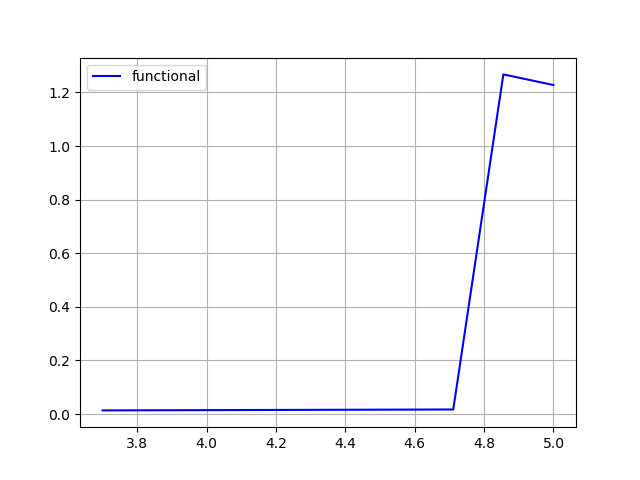
\includegraphics[scale=0.5]{fig/functional_3_7-5_5.png}
%\caption{$\alpha_3 \in [3.7, 5]$, угол в $5^{\circ}$}
%\end{figure}
%\end{frame}

%\begin{frame}{Примеры численного решения для поворотов на малые углы - первый случай, когда $\alpha_1$ и $\alpha_2$ фиксированы}
%\begin{figure}[H]
%\center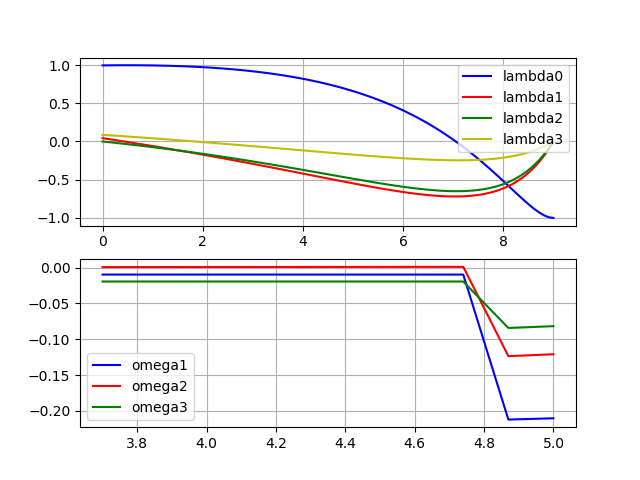
\includegraphics[scale=0.5]{fig/ivp_and_control_3_7-5_5.png}
%\caption{$\alpha_3 \in [3.7, 5]$, угол в $5^{\circ}$}
%\end{figure}
%\end{frame}

\begin{frame}{Пример численного решения для поворота на малый угол, когда $\alpha_1$ и $\alpha_3$ фиксированы}
\begin{figure}[H]
\center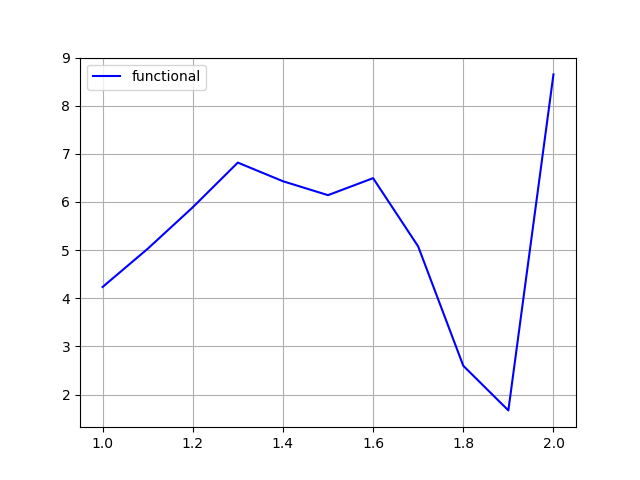
\includegraphics[scale=0.5]{fig/functional_alpha2_1-2_5.png}
\caption{$\alpha_2 \in [1, 2]$, угол в $5^{\circ}$}
\end{figure}
\end{frame}

\begin{frame}{Пример численного решения для поворота на малый угол, когда $\alpha_1$ и $\alpha_3$ фиксированы}
\begin{figure}[H]
\center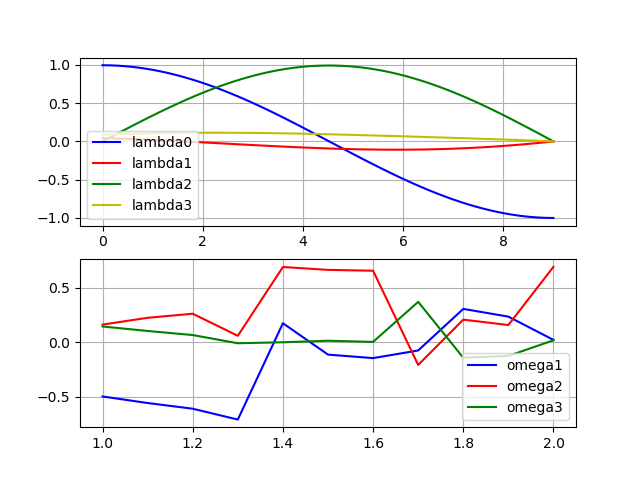
\includegraphics[scale=0.5]{fig/ivp_and_control_alpha2_1-2_5.png}
\caption{$\alpha_2 \in [1, 2]$, угол в $5^{\circ}$}
\end{figure}
\end{frame}

%\begin{frame}
%\frametitle{Примеры численного решения для поворотов на большие углы - третий случай, когда $\alpha_1$ и $\alpha_2$ фиксированы}
%\begin{figure}[H]
%\center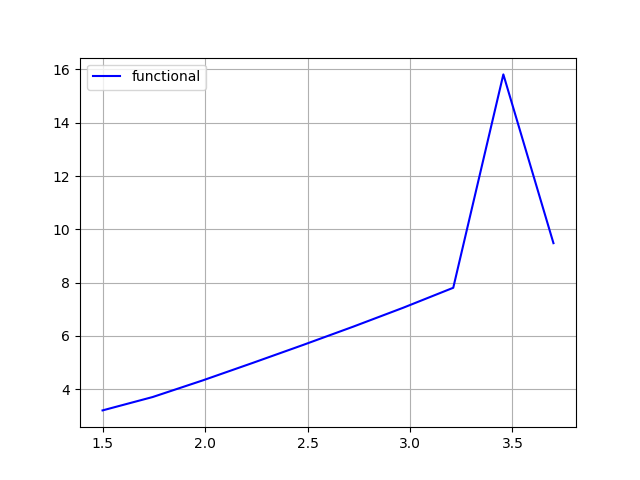
\includegraphics[scale=0.5]{fig/functional_1_5-3_7_50.png}
%\caption{$\alpha_3 \in [1.5, 3.7]$, угол в $50^{\circ}$}
%\end{figure}
%\end{frame}

%\begin{frame}{Примеры численного решения для поворотов на большие углы - третий случай, когда $\alpha_1$ и $\alpha_2$ фиксированы}
%\begin{figure}[H]
%\center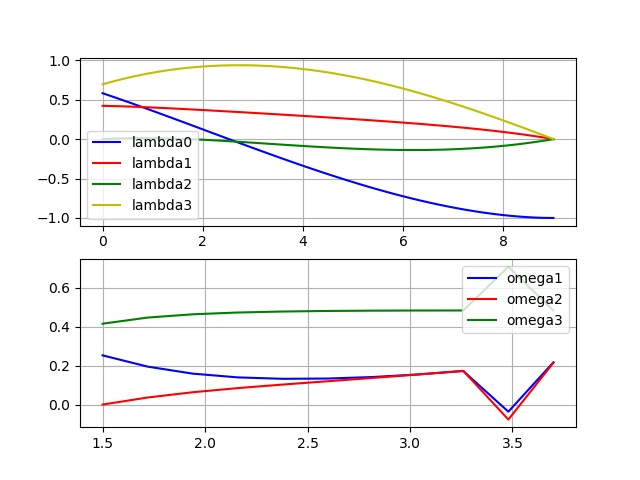
\includegraphics[scale=0.5]{fig/ivp_and_control_1_5-3_7_50.png}
%\caption{$\alpha_3 \in [1.5, 3.7]$, угол в $50^{\circ}$}
%\end{figure}
%\end{frame}

\begin{frame}{Пример численного решения для поворота на большой угол, когда $\alpha_1$ и $\alpha_3$ фиксированы}
\begin{figure}[H]
\center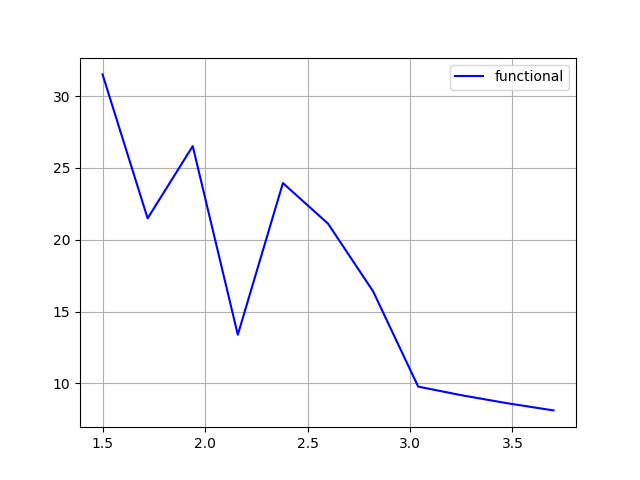
\includegraphics[scale=0.5]{fig/functional_alpha2_1_5-3_7_50.png}
\caption{$\alpha_2 \in [1.5, 3.7]$, угол в $50^{\circ}$}
\end{figure}
\end{frame}

\begin{frame}{Пример численного решения для поворота на большой угол, когда $\alpha_1$ и $\alpha_3$ фиксированы}
\begin{figure}[H]
\center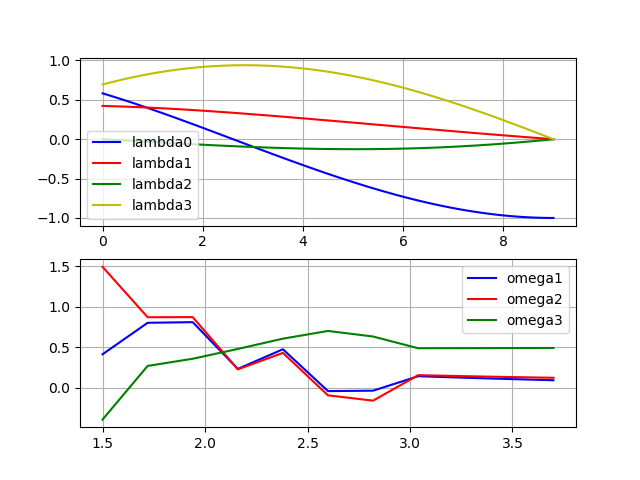
\includegraphics[scale=0.5]{fig/ivp_and_control_alpha2_1_5-3_7_50.png}
\caption{$\alpha_2 \in [1.5, 3.7]$, угол в $50^{\circ}$}
\end{figure}
\end{frame}

\begin{frame}{База данных для хранения графиков}
\begin{figure}[H]
\center
\includegraphics[scale=0.5]{fig/MongoDB-Logo.png}
\center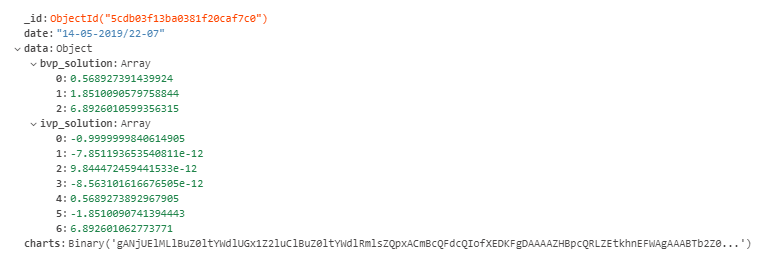
\includegraphics[scale=0.5]{fig/mongo_results.png}
\caption{Пример документа с результатами}
\end{figure}
\end{frame}

\begin{frame}[standout]
Спасибо за внимание!
\end{frame}

\end{document}
